% This text is released under the Creative Commons Attribution-NonCommercial-ShareAlike 4.0 International (CC BY-NC-SA 4.0) License
% Full license available at https://creativecommons.org/licenses/by-nc-sa/4.0/legalcode
% !TeX program = LuaLaTeX
\documentclass[12pt,a4paper,oneside]{article}
\usepackage[utf8]{inputenc} 
\usepackage[left=0cm,right=0cm,top=0cm,bottom=0cm,a4paper]{geometry}
\usepackage[parfill]{parskip}
\usepackage{epstopdf} %.eps file import
\usepackage{fontspec} %Fonts
    \setmainfont{ClearSans-Regular.ttf}[
        Path		   = fonts/clear-sans/,
        BoldFont       = ClearSans-Bold.ttf,
        ItalicFont     = ClearSans-Italic.ttf,
        BoldItalicFont = ClearSans-BoldItalic.ttf
    ]
    \setmonofont{LiberationMono-Regular.ttf}[
        Path 		   = fonts/liberation-mono/,
        BoldFont	   = LiberationMono-Bold.ttf,
        ItalicFont	   = LiberationMono-Italic.ttf,
        BoldItalicFont = LiberationMono-BoldItalic.ttf
    ]
    \newfontfamily\openiconic{open-iconic}[Path = fonts/]
    \newfontfamily\devicon{devicon}[Path = fonts/]
    \newfontfamily\chicago{ChicagoFLF.ttf}[Path = fonts/chicago/]
    \newfontfamily{\industrial}[
    	Path = fonts/industrial/, 
    	ItalicFont = Industrial-Italic.otf]
    	{Industrial-Regular.otf}
    \newcommand{\icon}[2]{\raisebox{-0.175\height}{\textcolor{#1}{\openiconic{#2}}}}
\usepackage{ragged2e} %text alignment
\usepackage[table,xcdraw,usenames,dvipsnames]{xcolor}
    \definecolor{code-background}{HTML}{f3f3f3}
    \definecolor{dark}{HTML}{31363b}
    \definecolor{linegrey}{HTML}{a8abaf}
    \definecolor{textgrey}{HTML}{777777}
    \definecolor{codekeyword1}{HTML}{3aa3ff}
\usepackage{colortbl}
\usepackage{float}
\usepackage{graphicx}
\usepackage{tabularx}
    \newcolumntype{R}{>{\raggedleft\let\newline\\\arraybackslash\hspace{0pt}}X}
\usepackage{verbatimbox}
\usepackage{soul}
    \sethlcolor{code-background}
\usepackage[skins]{tcolorbox}
    \tcbset{commonstyle/.style={boxrule=0pt,sharp corners,enhanced,nobeforeafter,boxsep=0pt,colback=code-background,fit width from 0 to \textwidth}}
    \newtcolorbox{codesnippetbox}[1][]{commonstyle,#1}
\usepackage{enumitem}
\usepackage[bottom]{footmisc}
\usepackage{url}
\usepackage{hyperref} % Hyperlink references
    \hypersetup{colorlinks=true,linkcolor=dark,urlcolor=MidnightBlue,pdfborder=0 0 0}
\usepackage{environ}
\usepackage[pages=some]{background}
%\usepackage{memoir}
\usepackage{mdframed} % minipage box
    \newmdenv{allborders}
    \newmdenv[topline=false,leftline=false,rightline=false,linecolor=linegrey]{bottomborder}
    \newmdenv[topline=false,leftline=false,rightline=false,linecolor=dark,backgroundcolor=dark,fontcolor=white]{headerborder}
    \mdfdefinestyle{titlebox}{
		leftline=false,
    	rightline=false,
    	innertopmargin=2mm,
    	innerbottommargin=2mm,
    	linewidth=1pt,
    	backgroundcolor=dark, 
    	fontcolor=white, 
    	linecolor=white
    }
    \mdfdefinestyle{commentbox}{
        topline=false,
        rightline=false,
        bottomline=false,
        linewidth=1mm,
        linecolor=linegrey,
        splittopskip=0,
        splitbottomskip=0,
        frametitleaboveskip=0,
        frametitlebelowskip=0,
        skipabove=0,
        skipbelow=0,
        leftmargin=+0.3cm,
        rightmargin=0,
        innertopmargin=2mm,
        innerbottommargin=2mm,
        roundcorner=0mm,
        backgroundcolor=white
    }
    \mdfdefinestyle{codebox}{
        topline=false,
        rightline=false,
        leftline=false,
        bottomline=false,
        splittopskip=0,
        splitbottomskip=0,
        frametitleaboveskip=0,
        frametitlebelowskip=0,
        skipabove=0,
        skipbelow=0,
        leftmargin=0,
        rightmargin=0,
        innertopmargin=2mm,
        innerbottommargin=2mm,
        roundcorner=0mm,
        backgroundcolor=code-background
    }
\usepackage{listings} %for code
    \lstset{ %
        backgroundcolor=\color{code-background},
        basicstyle=\scriptsize,
        breakatwhitespace=false,         % sets if automatic breaks should only happen at whitespace
        breaklines=true,                 % sets automatic line breaking
        commentstyle=\color{grey},   	   % comment style
        frame=single,                    % adds a frame around the code
        keepspaces=true,                 % keeps spaces in text, useful for keeping indentation of code (possibly needs columns=flexible)
        keywordstyle=\color{Violet},       % keyword style
        %numbers=left,                    % where to put the line-numbers; possible values are (none, left, right)
        %numbersep=5pt,                   % how far the line-numbers are from the code
        %numberstyle=\tiny\color{gray}, % the style that is used for the line-numbers
        %rulecolor=\color{black},         % if not set, the frame-color may be changed on line-breaks within not-black text (e.g. comments (green here))
        %stepnumber=1,                    % the step between two line-numbers. If it's 1, each line will be numbered
        tabsize=4,
        title=\lstname                   % show the filename of files included with \lstinputlisting; also try caption instead of title
    }
%%% Header %%%
\newenvironment{headersection}{\begin{headerborder}\vspace{0.5cm}\begin{minipage}[t]{\textwidth}}{\end{minipage}\vspace{0.5em}\end{headerborder}}
%%% Code snippets and terminal command snippets %%%
\newcommand{\code}[1]{\begin{small}\texttt{\sethlcolor{code-background}\hl{#1}}\end{small}} %Code text formatting
\newcommand{\terminalcmd}[1]{\begin{tabularx}{\textwidth}{cX}\textcolor{orange}{\$} & \code{#1}\end{tabularx}} %Terminal line formatting
%%% Blocks %%%
\newcommand{\blockheader}[1]{\raggedright{\textbf{\textcolor{textgrey}{#1}}\linebreak}}
\newcommand{\block}[1]{\begin{mdframed}[style=commentbox]\color{dark}{#1}\end{mdframed}}
\newenvironment{blocksection}{\begin{mdframed}[style=commentbox]\color{dark}}{\end{mdframed}}
\newenvironment{codeblock}{\begin{mdframed}[style=codebox]\color{dark}\small\ttfamily}{\par\end{mdframed}}
%%% Custom hrefs %%%
\newcommand{\cref}[3]{\href{#2}{\color{#1}{#3}}}%
%%% Custom free bullet point
\newcommand{\cbullet}[1]{\hangindent=0.57em{· #1}}
%\usepackage{showframe}

\color{dark}
\backgroundsetup{
	scale=1,
	color=dark,
	opacity=1,
	angle=0,
	contents={%
		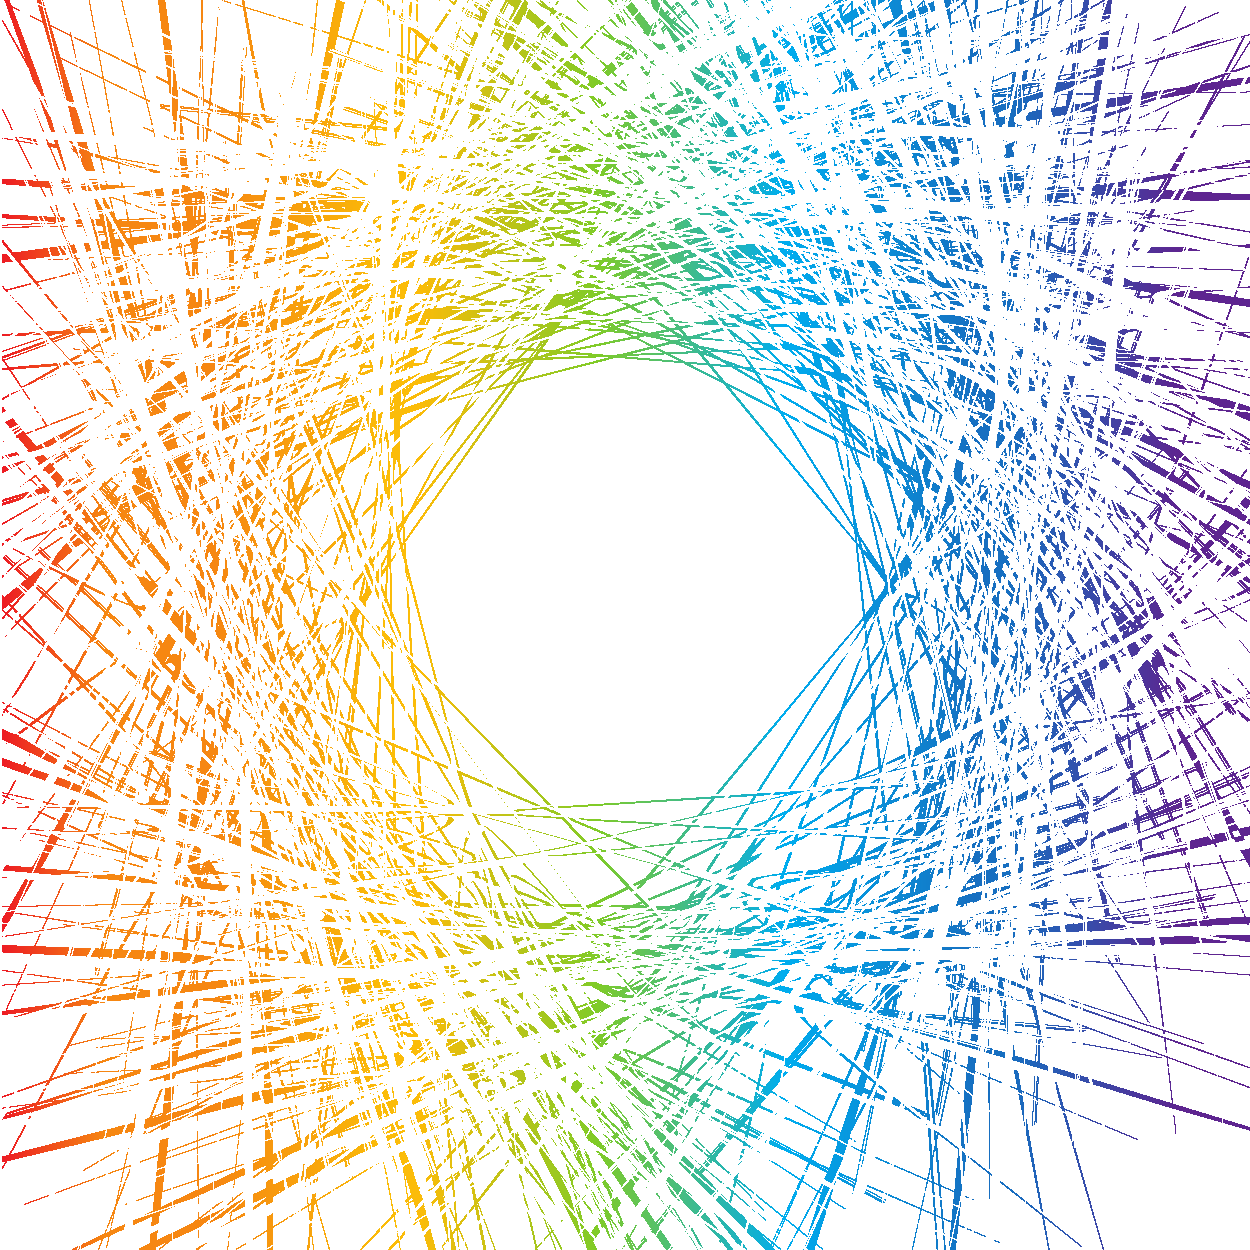
\includegraphics[width=\paperwidth,height=\paperheight]{img/Burst.pdf}
	}%
}
\setlength{\parindent}{0em}
\setlength{\parskip}{0.5em}
\renewcommand{\baselinestretch}{1.2}

\begin{document}
\pagecolor{dark}
\color{white}
%\BgThispage
\sloppy
\centering
\vspace*{0.5em}
\begin{tabularx}{0.95\linewidth}{lR}
	\cref{white}{https://an7ar35.bitbucket.io/}{\raisebox{-0.25\height}{
\includegraphics[scale=0.25]{common/avatar.png}} An7ar35} & 
	December 2017
\end{tabularx}

\vspace*{\fill}

\includegraphics[height=10em]{img/ArchMBP.pdf}\linebreak
\begin{mdframed}[style=titlebox]
	\centering
	\begin{Huge}
	    \industrial{Arch Linux installation guide\linebreak
	    for\linebreak
	    MacBook Pro Retina mid 2015 model}\par
	\end{Huge}
\end{mdframed}
\vspace*{2em}

\includegraphics[height=5em]{img/kde-logo.pdf}with KDE\par
\vspace*{\fill}
\begin{tabularx}{0.95\textwidth}{lR}
	& 
\includegraphics[height=3em]{common/licenses/by-nc-sa_eu.pdf}
\end{tabularx}
\vspace*{2em}

\newgeometry{left=1cm,right=1cm,top=1cm,bottom=1.5cm}
\setcounter{page}{1}
\pagecolor{white}
\color{dark}
\normalsize\justify
\tableofcontents
\clearpage

\section{Forewords}

After lots of reading, searching, experimenting, furious late-night shell command typing and 
do-overs here are the results of replacing OSX with Arch Linux (KDE) on a mid-2015 MacBook Pro. 

I would also advise backing up your drive using a complete bit-to-bit cloning process (unlike me, casually forgetting that step...) so that you retain a copy of everything including the recovery partition on the Mac. This way it is a one-step process to restore everything.

This guide assumes a basic working knowledge of Linux command line (bash).

\section{Nomenclatures}

\begin{tabularx}{\textwidth}{lX}
	\code{package-name} & Standard package \href{https://www.archlinux.org/packages/}{repository} - use \code{pacman} to install.\\
	\code{package-name}\textsuperscript{AUR} & Arch User Repository package (\href{https://aur.archlinux.org/}{AUR}) - use \code{yaourt} to install.\\
	\textcolor{orange}{\$} \code{...} & Command to type in at the command line prompt.
\end{tabularx}

\section{Machine Specs}

\begin{tabularx}{\textwidth}{|c|X|}
	\hline
	Display   & \cbullet{15.4" LED-backlit Retina display with IPS technology; 2880-by-1800 native resolution at 220 pixels per inch with support for millions of colours} \\\hline
	Processor & \cbullet{2.5GHz quad-core Intel Core i7 processor (Turbo Boost up to 3.7GHz) with 6MB shared L3 cache} \\\hline
	RAM       & · 16GB of 1600MHz DDR3L memory \\\hline
	GPU       & · Intel Iris Pro Graphics, \newline
				· AMD Radeon R9 M370X with 2GB of GDDR5 memory\\\hline
	Storage   & · 512GB PCIe-based flash \\\hline
	Webcam    & · 720p FaceTime HD camera \\\hline
	Network   & · 802.11ac Wi‑Fi wireless networking; IEEE 802.11a/b/g/n compatible, \newline
			    · Bluetooth 4.0 wireless technology \\
	\hline
\end{tabularx}

\section{Results}

\begin{small}\fcolorbox{linegrey}{white}{
	\textcolor{textgrey}{\textbf{Legend: }}
	\raisebox{-0.2\height}{\color{green}{\openiconic[]}} Works out-of-the-box or with few steps, 
	\raisebox{-0.2\height}{\color{blue}{\openiconic[]}} Requires some work, 
	\raisebox{-0.2\height}{\color{orange}{\openiconic[]}} Not fully working, 
	\raisebox{-0.2\height}{\color{red}{\openiconic[]}} Broken.}
\end{small}

//TODO

\begin{center}
	\rowcolors{2}{gray!25}{white}
	\begin{tabular}{lcl}
		\rowcolor{white!50}
		\textbf{Item} & \textbf{Result} & \textbf{Note}\\
		\hline\hline
		Wifi\footnotemark[1] & \raisebox{-0.2\height}{\color{green}{\openiconic[]}} & Works out-of-the-box, some error messages.\\
		Bluetooth & \raisebox{-0.2\height}{\color{green}{\openiconic[]}} & Uses standard \code{bluez} package.\\
		Display (IPS scaling)\footnotemark[2] & \raisebox{-0.2\height}{\color{orange}{\openiconic[]}} & Mixed results without Wayland\\
		Display (Backlight) & \raisebox{-0.2\height}{\color{blue}{\openiconic[]}} & Needs special EFI addon.\\
		AMD Radeon R9 M370X & \raisebox{-0.2\height}{\color{green}{\openiconic[]}} & Open source driver works like a charm\\
		Intel Iris Pro Graphics\footnotemark[3] & \raisebox{-0.2\height}{\color{red}{\openiconic[]}} & Disabled by default, graphic switching not working.\\
		Audio & \raisebox{-0.2\height}{\color{green}{\openiconic[]}} & Uses ALSA.\\
		FaceTimeHD camera & \raisebox{-0.2\height}{\color{orange}{\openiconic[]}} & Requires own driver construction\\
		Keyboard & \raisebox{-0.2\height}{\color{green}{\openiconic[]}} & ISO layout in command line but perfect in KDE.\\
		Keyboard (Backlight) & \raisebox{-0.2\height}{\color{green}{\openiconic[]}} & Works out-of-the-box.\\
		Keyboard \fbox{Fn} keys & \raisebox{-0.2\height}{\color{green}{\openiconic[]}} & Works out-of-the-box in KDE.
	\end{tabular}
\end{center}

\footnotetext[1]{Error messages with default kernel module but doesn't seem to affect connections.}
\footnotetext[2]{A workable solution can be setting the resolution to 1920x1200. The scale is good for a 15" screen.}
\footnotetext[3]{Being stuck with using the dedicated GPU means that the battery will drain faster than when using Intel's IGU.}

//Heating issues with mbp, fan control and turning off boost on the processor to keep things
reasonable temperature-wise.

\section{How-To}

\subsection{Packages}

For complete guides refer to the \code{pacman} \href{https://wiki.archlinux.org/index.php/Pacman}{Wiki} and \code{yaourt}  \href{https://archlinux.fr/yaourt-en}{Wiki}.

\begin{tabularx}{\textwidth}{lX}
	\code{pacman -Syuu} & Updates cache and packages installed with \code{pacman}.\\
	\code{pacman -S package-name} & Installs \code{package-name}.\\
	\code{pacman -R package-name} & Removes \code{package-name}.
\end{tabularx}

\section{Pre-Installation}

\subsection{Preparations}

\textbf{Backup drive} (complete drive clone preferable).

Make a copy of the colour profile file(s) on the mac to a USB stick. It will be useful later on Linux. The profiles are located in \code{/Library/ColorSync/Profiles/Displays/*}.

\subsection{Making a bootable USB}

\subsubsection{From Linux}

\terminalcmd{dd if=archlinux.iso of=/dev/sdX bs=16M \&\& sync}
\block{Where \code{X} is your target USB drive letter (use \code{lsblk} for an overview of all connected drives to find out)}

\subsubsection{From a Mac}

\terminalcmd{diskutil unmountDisk diskX}
\block{Where \code{X} is your target USB drive number (use \code{diskutil list} for an overview of all connected drives to find out).}
\terminalcmd{sudo dd if=/Users/\$USERNAME/Downloads/archlinux.iso of=/dev/diskX bs=16M}
\block{Replace \code{\$USERNAME} with your username on the mac and replace \code{X} with the USB drive's number.}

\section{Installation}

\subsection{Booting from the USB stick}

Simply plug in the USB in the MBP and press the \fbox{Alt} (a.k.a. \fbox{options}) key during start up
to reach the boot menu.

\subsection{Preliminary setup}

\terminalcmd{loadkeys uk}
\block{Load your keyboard layout. Replace `uk` with whichever you have on your machine.}
\terminalcmd{wifi-menu}
\block{Connect up to the wifi network. On the MPB Pro 2015 the wifi gets detected and works out of the box at this stage.}

\subsection{Partitioning and Crypto volume setup}

The assumption here is that the hard drive where everything will be installed to is \code{/dev/sda}. The partition structure will thus be: \\
\code{/dev/sda1} for the EFI partition,\\
\code{/dev/sda2} for the Boot partition and\\
\code{/dev/sda3} for the encrypted volume where the root, home and swap will be located.\\

\terminalcmd{cgdisk /dev/sda}
\begin{blocksection}
	\blockheader{Partition layout with just Linux}
	\textit{Warning: this will erase every thing including the recovery partition for OSX. \\
	No easy way to go back after this without a bit-to-bit HDD clone}
	\begin{enumerate}
 		\item 100M partition `EFI' (Hex \#\code{ef00})
	 	\item 250M partition `Boot' (Hex \#\code{8300})
	 	\item 100\% remainder of the space for the crypto volume (Hex \#\code{8300})
	\end{enumerate}
	The root and home partition will be created later in the crypto volume
\end{blocksection}
\terminalcmd{cryptsetup --verbose --verify-passphrase --cipher aes-xts-plain64 --key-size 512 --hash sha512 --iter-time 5000 --use-random luksFormat /dev/sda3}
	\block{Sets up the crypto volume.}
\terminalcmd{cryptsetup open --type luks /dev/sda2 mctoasty}
	\block{\code{mctoasty} is the mounted name of the crypto volume. Can be changed to whatever is preferred.}

\subsubsection{Create crypto volume partitions}

\terminalcmd{pvcreate /dev/mapper/mctoasty}
\terminalcmd{vgcreate vg0 /dev/mapper/mctoasty}
\terminalcmd{lvcreate --size 16G vg0 --name swap}
    \block{Generally swap size value is set to the amount of RAM.}
\terminalcmd{lvcreate --size 50GB vg0 --name root}
	\block{Adjust root's size as required.}
\item \terminalcmd{lvcreate -l +100\%FREE vg0 --name home}
    \block{Creates the home parition with the remainder of the free space.}

\subsubsection{Formatting all the partitions}

\terminalcmd{mkfs.vfat -F32 /dev/sda1}
	\block{EFI partition}
\terminalcmd{mkfs.ext2 /dev/sda2}
	\block{Boot partition}
\terminalcmd{mkswap /dev/mapper/vg0-swap}
\terminalcmd{mkfs.ext4 /dev/mapper/vg0-root}
\terminalcmd{mkfs.ext4 /dev/mapper/vg0-home}

\subsubsection{Mount all the partitions}

\terminalcmd{mount /dev/mapper/vg0-root /mnt}
\terminalcmd{swapon /dev/mapper/vg0-swap}
\terminalcmd{mkdir /mnt/boot}
\terminalcmd{mount /dev/sda2 /mnt/boot}
\terminalcmd{mkdir /mnt/boot/efi}
\terminalcmd{mount /dev/sda1 /mnt/boot/efi}
\terminalcmd{mkdir /mnt/home}
\terminalcmd{mount /dev/mapper/vg0-home /mnt/home}

\section{System Setup I: Base System Installation}

\terminalcmd{pacstrap /mnt base base-devel grub-efi-x86\_64 git efibootmgr bash-completion dialog wpa\_supplicant}
\begin{blocksection}
    Base packages along with GRUB and the EFI boot manager, git (will be useful later), bash completion and the stuff needed to keep the Wifi device in working order after reboot.
\end{blocksection}

\subsection{Generating fstab}

\terminalcmd{genfstab -pU /mnt >> /mnt/etc/fstab}
\begin{blocksection}
    \blockheader{Important!}
    This generates the fstab. i.e.: It saves our mounted partitions and swap configuration for persistence after a reboot. If you miss this step you'll have to reboot with the USB, mount everything again and then generate the fstab file.
\end{blocksection}
\terminalcmd{arch-chroot /mnt /bin/bash}

\subsection{System clock}

\terminalcmd{ln -s /usr/share/zoneinfo/\$ZONE/\$REGION /etc/localtime}
\begin{blocksection}
    Replace \textcolor{codekeyword1}{\$ZONE} with yours from \code{/usr/share/zoneinfo/}\\
    Replace \textcolor{codekeyword1}{\$REGION} with yours from \code{/usr/share/zoneinfo/\$ZONE/}\\
    e.g.: \code{/usr/share/zoneinfo/Europe/London}
\end{blocksection}
\terminalcmd{hwclock --systohc --utc}

\subsection{Hostname}

\terminalcmd{echo \$HOSTNAME > /etc/hostname}
\terminalcmd{nano /etc/hosts}
\begin{blocksection}
    Add the hostname at the end of each of the relevant lines in this file for completion's sake. Replace \textcolor{codekeyword1}{\$HOSTNAME} by the hostname you want to computer to have.
\end{blocksection}

\subsection{Basic fonts}

\terminalcmd{pacman -S terminus-font ttf-dejavu ttf-liberation}
\begin{blocksection}
    The terminus font will be used to make the console font more \href{https://wiki.archlinux.org/index.php/HiDPI#Linux_console}{readable} on the HiDPI display.
\end{blocksection}

\subsection{Locale}

\terminalcmd{locale-gen}
    \block{Generates the locale file}
\terminalcmd{nano /etc/local.conf}
    \block{Edit the locale configuration and delete the hash in front of the desired locale.}
\terminalcmd{local-gen}
    \block{Needs to run again to apply the changes made in the previous step.}
\terminalcmd{nano /etc/locale.conf}
\begin{blocksection}
    To set permanent locale settings add the lines:\\
    \begin{codeblock}
        LANG=en\_GB.UTF-8\\
        LANGUAGE=en\_GB\\
        LC\_ALL=C
    \end{codeblock}
\end{blocksection}

\subsection{Console keymap and font}

To see a list of all available keymaps: \code{find /usr/share/kbd/keymaps/ -type f | more}\\
To see a list of all installed console fonts: \code{ls /usr/share/kbd/consolefonts/}\\
For font maps check the \href{https://wiki.archlinux.org/index.php/fonts#Persistent_configuration}{Arch Wiki} and the \href{https://en.wikipedia.org/wiki/ISO/IEC_8859#The_parts_of_ISO/IEC_8859}{Wikipedia} entries.

\terminalcmd{nano /etc/vconsole.conf}
\begin{blocksection}
    To set permanent setting for the console add the lines:\\
    \begin{codeblock}
    KEYMAP=uk\\
    FONT=ter-228n\\
    FONT\_MAP=8859-1
    \end{codeblock}
\end{blocksection}

\subsection{Root/User Accounts}

\terminalcmd{passwd}
    \block{Set the root password.}
\terminalcmd{useradd -m -g users -G wheel -s /bin/bash \$USERNAME}
    \block{Adds a user. Replace \$USERNAME with whatever user name you which to use.}
\terminalcmd{passwd \$USERNAME}
    \block{Sets the user's password.}

\subsection{Initial RAM Environment Configuration [\href{https://wiki.archlinux.org/index.php/mkinitcpio}{\texttt{mkinitcpio}}]}

\terminalcmd{nano /etc/mkinitcpio.conf}
\begin{blocksection}
    In the file do the following:
    \begin{itemize}[noitemsep,topsep=0pt,leftmargin=*]
        \item In 'MODULES:
        \begin{enumerate}
            \item Add `ext4`
        \end{enumerate}
        \item In 'HOOKS':
        \begin{enumerate}
            \item Add \code{encrypt} and \code{lvm2} before \code{filesystems}
            \item Add \code{consolefont} right after \code{autodetect}\\
                  (to avoid squinting at the crypto volume password prompt)
            \item Move \code{keyboard} right after \code{consolefont}
        \end{enumerate}
    \end{itemize}
    HOOKS should be ordered as such in the end:\\
    \code{HOOKS=(base udev autodetect consolefont keyboard modconf block encrypt lvm2 filesystems fsck)}
\end{blocksection}
        
\terminalcmd{mkinitcpio -p linux}
    \block{Regenerates the initrd image.}

\subsection{GRUB boot loader}

\terminalcmd{grub-install}
\terminalcmd{nano /etc/default/grub}
\begin{blocksection}
    At line with \code{GRUB\_CMDLINE\_LINUX} add the arguments so that it becomes\\
    \code{GRUB\_CMDLINE\_LINUX="cryptdevice=/dev/sda3:luks:allow-discards"}
\end{blocksection}
\terminalcmd{grub-mkconfig -o /boot/grub/grub.cfg}

\subsection{Dismount and reboot}

\terminalcmd{umount -R /mnt}
\terminalcmd{swapoff -a}

Remove the USB stick then \code{reboot}.

\textbf{Note}: If you want a break this is the place to take it. Instead of rebooting just shutdown the machine.

\section{System Setup II: Hardware and Tools}

Reconnect to your wifi with \code{sudo wifi-menu}

\subsection{Enabling the multilib package repository}

\terminalcmd{nano /etc/pacman.conf}
\begin{blocksection}
    Uncomment the multilib lines (i.e. remove the leading \code{\#}):
    \begin{codeblock}
        \#[multilib]\\
        \#Include = /etc/pacman.d/mirrorlist
    \end{codeblock}
\end{blocksection}
\terminalcmd{pacman -Syuu}
    \block{Updates the cache}

\subsection{AUR package manager}

From your home directory (\code{cd \textasciitilde}):

\terminalcmd{mkdir -p git-repos/system-builds}
\terminalcmd{cd git-repos/system-builds}
    \block{Or whatever directory chosen to clone the repositories into.}
\terminalcmd{git clone https://aur.archlinux.org/package-query.git}
    \block{Required for \href{https://github.com/archlinuxfr/yaourt}{Yaourt}}
\terminalcmd{git clone https://aur.archlinux.org/yaourt.git}
    \block{Easy AUR package installations from the console.}

For each of the 2 packages, \code{cd} into their respective directories and run the following command to install:

\terminalcmd{makepkg -si}
    \block{e.g.: \code{cd package-query} then \code{makepkg -si}}

\subsection{Console-Fu}

\terminalcmd{yaourt -S hstr-git}
    \block{This is a replacement on \href{https://github.com/dvorka/hstr}{steroids} for the console's \fbox{ctrl}+\fbox{r}}
\terminalcmd{hh --show-configuration >> ~/.bashrc}
    \block{Adds the config options for HSTR to your bash profile and auto-starts hh on login.}
\terminalcmd{pacman -S powertop htop}
    \block{Installs 2 of the most basic and useful monitoring tools in linux.}
    
\subsection{Power management}

\terminalcmd{yaourt -S laptop-mode-tools}
    \block{All the laptop-centric \href{https://wiki.archlinux.org/index.php/Laptop_Mode_Tools}{power saving} goodies}
\terminalcmd{sudo systemctl enable laptop-mode.service}
    \block{Turns on the service} 
\terminalcmd{pacman -S acpid}
    \block{\emph{(Optional)} \href{https://wiki.archlinux.org/index.php/Acpid}{Daemon} for delivering ACPI events.}

\subsection{Hardware}

\subsubsection{Fans}

\terminalcmd{yaourt -S macfanctld}
    \block{\href{https://github.com/MikaelStrom/macfanctld}{macfanctld}\textsuperscript{AUR} controls the mbp fans.}
\terminalcmd{sudo systemctl enable macfanctld.service}
    \block{Turns on the service}

\subsubsection{Processor}

\terminalcmd{pacman -S intel-ucode}
    \block{For intel's \href{https://wiki.archlinux.org/index.php/microcode}{microcode} update.}
\terminalcmd{grub-mkconfig -o /boot/grub/grub.cfg}
    \block{Need to update grub so that it loads the Microcode updates at boot}
\terminalcmd{yaourt -S msr-tools}
    \block{\href{https://01.org/msr-tools}{MSR-Tools} will be used to turn off boost on the processor from a script.}
    
\subsubsection{Sound}

\href{https://wiki.archlinux.org/index.php/ALSA}{Alsa} works without issues.

\terminalcmd{sudo pacman -S alsa-utils alsa-plugins}
\terminalcmd{alsamixer}
\begin{blocksection}
    Make sure your current sound card is the "HDA Intel PCH" and that your master volume is up and unmuted (mute=MM, unmuted=00 at the bottom of the volume bar. You can use the \fbox{M} key on the keyboard to toggle mute).
\end{blocksection}
\terminalcmd{speaker-test -c 2}
    \block{To make sure the sound works.}


\textbf{Note}: The internal speaker might not be disabled when using the headphone jack. To solve this, enable "Auto-mute" in \code{alsamixer}.

\subsubsection{Bluetooth}

\href{https://wiki.archlinux.org/index.php/Bluetooth}{Bluetooth} works out-of-the-box with the standard packages.

\terminalcmd{sudo pacman -S bluez bluez-utils}
\terminalcmd{modprobe btusb}
\terminalcmd{sudo systemctl enable bluetooth.service}

\subsubsection{Video}
\terminalcmd{sudo pacman -S mesa xf86-video-amdgpu vulkan-radeon lib32-mesa}
\begin{blocksection}
    Installs the open source drivers for the ATI GPU along with the 32bit libs and the Vulkan drivers.\\
    The \href{https://wiki.archlinux.org/index.php/Lm_sensors}{\code{lm\_sensors}} package used for temperature monitoring is a dependency for \code{mesa} so will be installed with it.\\
    Run \code{sensors} to see all the temperatures.
\end{blocksection}
\terminalcmd{yaourt -S radeontop}
    \block{\emph{(Optional)} Monitoring utility for Radeon GPU cards.}

\subsubsection{Display brightness}

\href{https://github.com/0xbb/apple_set_os.efi}{link}

\href{https://github.com/Dunedan/mbp-2016-linux/issues/38}{link}
\href{https://bugzilla.kernel.org/show_bug.cgi?id=105051#c37}{link}
\href{https://bugzilla.kernel.org/show_bug.cgi?id=105051#c39}{link}

\subsubsection{Webcam}

The 2015 MBP has \href{https://wiki.archlinux.org/index.php/MacBook#Facetime_HD}{Facetime HD}.
Fortunately there is a reversed-engineered driver but "PC suspension is not supported if a 
program that is keeping the camera active is running".

DOES NOT WORK!

\terminalcmd{yaourt -S bcwc-pcie-git}

\subsubsection{Other Drivers}

Possible missing firmware module for:
\begin{itemize}[noitemsep,topsep=0pt,leftmargin=*]
    \item wd719x
    \item aic94xx
\end{itemize}

\terminalcmd{pacman -S aic94xx-firmware}
\terminalcmd{pacman -S wd719x-firmware}
\terminalcmd{sudo mkinitcpio -p linux}
    \block{To make sure drivers are loaded.}

\section{System Setup III: Desktop}

Wayland support as of Dec 2017 on KDE is beta at best. Scaling in nice but buggy as hell displaying artefacts. Until that gets a lot better Xorg is the default choice as display managers go even if HiDPI support is terrible. 

\subsection{Display manager (\href{https://wiki.archlinux.org/index.php/xorg}{Xorg})}

\terminalcmd{xorg, xorg-server xorg-xinit}

\subsection{Desktop Environment (\href{https://wiki.archlinux.org/index.php/KDE}{KDE})}

\subsubsection{What works}

\begin{itemize}[noitemsep,topsep=0pt,leftmargin=*]
    \item Keyboard and the backlight
    \item Bluetooth? //TODO check
\end{itemize}

\terminalcmd{sudo pacman -S plasma kde-applications sddm systemd-kcm}
\terminalcmd{sudo systemctl enable sddm.service}
\terminalcmd{sudo systemctl start sddm.service}

kde-thumbnailer-odf\\
kde-thumbnailer-epub\\
kde-thumbnailer-gimpsources\\


\href{https://wiki.archlinux.org/index.php/SDDM}{SDDM}

//TODO auto-login

\code{sudo systemctl enable NetworkManager.service} in KDE then restart to get wifi working on the desktop


\subsection{Printing/Scanning}

\terminalcmd{sudo pacman -S cups print-manager}
\terminalcmd{//TODO scanning}


\section{System Setup IV: Applications}

`flite` (missing packages causes a "text-to-speech" error - see `journalctl -b`)


\subsection{File system}

\code{ntfs-3g}
\code{exfat-utils}
\code{gparted} and/or \code{partitionmanager} (KDE)

\subsection{Firewall}

Install \code{firewalld} and start the \code{firewalld.service}

If there is a systemd timeout \href{https://bugzilla.redhat.com/show_bug.cgi?id=1294415#c10}{issue} on restart: 
\terminalcmd{sudo nano /etc/firewalld/firewalld.conf}
\begin{blocksection}
    Find the \code{CleanupOnExit} option in the file and set it to \code{no}:\\
    \code{CleanupOnExit=no}
\end{blocksection}

\subsection{Tools/Utils}

p7zip
unrar
Ark (GUI front end for compression)

\subsection{Fonts}

adobe-source-code-pro
adobe-source-sans-pro
adobe-source-serif-pro
ttf-mac-fonts

\subsection{Console apps}

`cmus`
`wget`

\subsubsection{Development}

valgrind, cmake, clang, extra-cmake-modules, clang-tools-extra, 
sqlitebrowser

\subsection{Desktop apps}


\subsubsection{Pacman}

yakuake, thunderbird, firefox, cairo-dock, cairo-dock-plugins, deja-dup, truecrypt, veracrypt, 
redshift, plasma5-applets-redshift-control, 


\subsubsection{AUR (Yaourt)}

pamac-aur

//discord

\section{Bugs}

//TODO `kfd kfd: kgd2kfd\_probe failed` at start up

//TODO `brcmfmac: brcmf\_inetaddr\_changed: fail to get arp ip table err:-23` after wifi connect



\subsection{USB suspend error}

You may get the following sort of error after suspend/sleep:

\begin{codeblock}
    usb 2-4: usb\_reset\_and\_verify\_device Failed to disable LTM\\
    usb usb2-port4: cannot disable (err=-32)
\end{codeblock}

The Kernel \href{https://bugzilla.kernel.org/show_bug.cgi?id=117811}{Bug report \#117811}'s thread suggest disabling USB auto-suspend.

\begin{itemize}[noitemsep,topsep=0pt,leftmargin=*]
    \item If you are using [TLP](https://wiki.archlinux.org/index.php/TLP):\\
        \code{nano /etc/default/tlp} and set \code{USB\_AUTOSUSPEND=0}
    \item If you are \textbf{not} using \href{https://wiki.archlinux.org/index.php/TLP}{TLP}:\\
        \code{sudo echo on | tee /sys/bus/usb/devices/*/power/control}
\end{itemize}



\clearpage
\section{References}

\begin{itemize}
	\item \href{https://wiki.archlinux.org/index.php/MacBookPro11,x#Using_the_MacBook.27s_native_EFI_bootloader_.28recommended.29}{Arch Linux's MacBookPro 11.x Wiki page}
	\item \href{https://gist.github.com/mattiaslundberg/8620837}{Mattias Lindberg's Encrypted volume Arch install guide}
	\item \href{https://www.howtoforge.com/tutorial/how-to-install-arch-linux-with-full-disk-encryption/}{HowToForge | How to install Arch Linux with Full Disk Encryption}
\end{itemize}

\end{document}
